\documentclass[12pt, titlepage]{article}

\usepackage{fullpage}
\usepackage[round]{natbib}
\usepackage{multirow}
\usepackage{booktabs}
\usepackage{tabularx}
\usepackage{graphicx}
\usepackage{float}
\usepackage{hyperref}
\usepackage{verbatim}
\usepackage[normalem]{ulem}
\hypersetup{
    colorlinks,
    citecolor=black,
    filecolor=black,
    linkcolor=red,
    urlcolor=blue
}
\usepackage[round]{natbib}

\newcounter{acnum}
\newcommand{\actheacnum}{AC\theacnum}
\newcommand{\acref}[1]{AC\ref{#1}}

\newcounter{ucnum}
\newcommand{\uctheucnum}{UC\theucnum}
\newcommand{\uref}[1]{UC\ref{#1}}

\newcounter{mnum}
\newcommand{\mthemnum}{M\themnum}
\newcommand{\mref}[1]{M\ref{#1}}

\title{SE 3XA3: Software Requirements Specification\\Synergy Inventory Management System (SIMS)}

\author{Team \#33, 'Sick Ideas'
		\\ Nathan Coit - 400022342
		\\ Lucas Shanks - 400029943
		\\ Cameron Van Ravens - 400020215
}

\date{\today}

\begin{document}

\maketitle

\pagenumbering{roman}
\tableofcontents
\listoftables
\listoffigures

\begin{table}[bp]
\caption{\bf Revision History}
\begin{tabularx}{\textwidth}{p{3cm}p{2cm}X}
\toprule {\bf Date} & {\bf Version} & {\bf Notes}\\
\midrule
11/10/17 & 0.0 & Initial Revision\\
12/6/17 & 1.0 & Revision 1\\
\bottomrule
\end{tabularx}
\end{table}

\newpage

\pagenumbering{arabic}

\section{Introduction}

This is the software Requirement Specification guide for the Synergy Inventory Management System (SIMS) project. The purpose of this project is to create an open source Inventory Management System, giving small companies and warehouses a simple to use and cost effective inventory management platform.\\

Decomposing a system into modules is a commonly accepted approach to developing
software. Our group advocates a decomposition
based on the principle of information hiding. This
principle supports design for change, because the ``secrets'' that each module
hides represent likely future changes. Design for change is valuable when developing software,
where modifications are frequent, especially during initial development as the
solution space is explored.

Our design principle follows:
\begin{itemize}
\item System details that are likely to change independently should be the
  secrets of separate modules.
\item Each data structure is used in only one module.
\item Any other program that requires information stored in a module's data
  structures must obtain it by calling access programs belonging to that module.
\end{itemize}

The rest of the document is organized as follows. Section
\ref{SecChange} lists the anticipated and unlikely changes of the software
requirements. Section \ref{SecMH} summarizes the module decomposition that
was constructed according to the likely changes. Section \ref{SecConnection}
specifies the connections between the software requirements and the
modules. Section \ref{SecMD} gives a detailed description of the
modules. Section \ref{SecTM} includes two traceability matrices. One checks
the completeness of the design against the requirements provided in the SRS. The
other shows the relation between anticipated changes and the modules. Section
\ref{SecUse} describes the use relation between modules.

\section{Anticipated and Unlikely Changes} \label{SecChange}

During the design process for SIMS, design decisions made by the team members followed the principle of information hiding and designing for change. While the application will not likely stray from the original specifications, should an improved or new change arise, it will be easily implementable. The following sections lists possible changes to the relatively finalized functional implementation classified into two categories according to the likeliness of the change with Anticipated Changes located in Section \ref{SecAchange} and Unlikely Changes listed in Section \ref{SecUchange}.

\subsection{Anticipated Changes} \label{SecAchange}

During the design process, the design for change paradigm was used. Changes that are likely to happen to elements hidden in modules are identified as Anticipated Changes. These changes are easy to implement and do not affect the rest of the project. 

\begin{description}
\item[\refstepcounter{acnum} \actheacnum \label{ac1}:] The specific hardware on which the software is running.
\item[\refstepcounter{acnum} \actheacnum \label{ac2}:] The specific NodeJS, AngularJS, PostgreSQL and dependency versions
\item[\refstepcounter{acnum} \actheacnum \label{ac3}:] The standard web security protocols
\item[\refstepcounter{acnum} \actheacnum \label{ac4}:] Additional functionality of the inventory management system
\item[\refstepcounter{acnum} \actheacnum \label{ac5}:] The front-end interface design
\end{description}

\subsection{Unlikely Changes} \label{SecUchange}

Design decisions that are likely to affect the rest of the system are classified as unlikely to change. The following design decision are unlikely to change, due to the risk of having to change multiple modules.

\begin{description}
\item[\refstepcounter{ucnum} \uctheucnum \label{ucIO}:] Input/Output devices (Input: File and/or Keyboard, Output: File, Memory, and/or Screen).
\item[\refstepcounter{ucnum} \uctheucnum \label{ucInput1}:] There will always be a source of input data external to the software.
\item[\refstepcounter{ucnum} \uctheucnum \label{ucInput2}:] The database schema design
\item[\refstepcounter{ucnum} \uctheucnum \label{ucInput3}:] The inventory analytics algorithms
\item[\refstepcounter{ucnum} \uctheucnum \label{ucInput4}:] The overall purpose of the system: Providing an Inventory Management System
\end{description}

\section{Module Hierarchy} \label{SecMH}

This section provides an overview of the module design. Modules are summarized
in a hierarchy decomposed by secrets in Table \ref{TblMH}. The modules listed
below, which are leaves in the hierarchy tree, are the modules that will
actually be implemented.

\begin{description}
\item [\refstepcounter{mnum} \mthemnum \label{mH1}:] Hardware-Hiding Module*
\item [\refstepcounter{mnum} \mthemnum \label{mH2}:] Database Module
\item [\refstepcounter{mnum} \mthemnum \label{mH3}:] OS Validation Module
\item [\refstepcounter{mnum} \mthemnum \label{mH4}:] Data Validation Module
\item [\refstepcounter{mnum} \mthemnum \label{mH5}:] Data Query Module
\item [\refstepcounter{mnum} \mthemnum \label{mH6}:] User Authentication Module
\item [\refstepcounter{mnum} \mthemnum \label{mH7}:] GUI Data Retrieval Module
\item [\refstepcounter{mnum} \mthemnum \label{mH8}:] GUI Display Module
\end{description}
\textbf{Note*: Hardware Hiding is not a module implemented in SIMS since it is software based. The lowest level that the software interfaces with the OS. This module, although not in the design, was included for legacy purposes, as it is a part of the Parnas and Madey four-variable model.}


\begin{table}[h!]
\centering
\begin{tabular}{p{0.3\textwidth} p{0.6\textwidth}}
\toprule
\textbf{Level 1} & \textbf{Level 2}\\
\midrule

{Hardware-Hiding Module} & ~ \\
\midrule
\multirow{7}{0.3\textwidth}{Behaviour-Hiding Module} & \sout{OS Validation Module}\\
& GUI Display Module\\
& Data Validation Module\\
& Database Module\\
\midrule
\multirow{3}{0.3\textwidth}{Software Decision Module} & Data Query Module\\
& User Authentication Module\\
& GUI Data Retrieval Module\\
\bottomrule

\end{tabular}
\caption{Module Hierarchy}
\label{TblMH}
\end{table}

\section{Connection Between Requirements and Design} \label{SecConnection}

The design of the application is intended to satisfy the requirements developed in the SRS, more specifically designing for requirements. One example this can be seen in the implementation of user security in the non-functional requirements. From the requirement of allowing users to only view their own inventory and data and user security, with information hiding, designing for change, as well as security in mind, solutions can be created to protect each users personal information (password encryption, checking user authorization). \\

\noindent Further examples of the connection between the requirements and design can be found in in Table \ref{TblRT} showing connections between the requirements and modules. The system is designed to satisfy the requirements set in the SRS document.

\section{Module Decomposition} \label{SecMD}

The \emph{Secrets} field in module decomposition is a brief statement of the design decision hidden by the module. The \emph{Services} field specifies \emph{what} the module will do
without documenting \emph{how} to do it. For each module, a suggestion for the
implementing software is given under the \emph{Implemented By} title. If the
entry is \emph{OS}, this means that the module is provided by the operating
system or by standard programming language libraries.  \\

\noindent Only the leaf modules in the
hierarchy have to be implemented. If a dash (\emph{--}) is shown, this means
that the module is not a leaf and will not have to be implemented. Whether or
not this module is implemented depends on the programming language
selected.

\subsection{Behaviour-Hiding Module}

\begin{comment}
\begin{description}
\item[Secrets:]The contents of the required behaviours.
\item[Services:]Includes programs that provide externally visible behaviour of
  the system as specified in the software requirements specification (SRS)
  documents. This module serves as a communication layer between the
  hardware-hiding module and the software decision module. The programs in this
  module will need to change if there are changes in the SRS.
\item[Implemented By:] SIMS
\end{description}
\end{comment}

\subsubsection{Database Module (\mref{mH2})}
\begin{description}
\item[Secrets:]The format and structure of the save data.
\item[Services:] Stores/outputs user inventory data.
\item[Implemented By:] SIMS
\end{description}

\subsubsection{OS Validation Module (\mref{mH3})}
\begin{description}
\item[Secrets:]The algorithms determining how to set the proper file path.
\item[Services:]Determines user OS and configures file paths accordingly
\item[Implemented By:] SIMS
\end{description}

\subsubsection{Data Validation Module (\mref{mH4})}
\begin{description}
\item[Secrets:]The rules for the input: accepts valid input data.
\item[Services:]Converts the input data into the data structure used by the
  input parameters module.
\item[Implemented By:] SIMS
\end{description}

\subsubsection{GUI Display Module (\mref{mH8})}
\begin{description}
\item[Secrets:]The rules for the display: mapping the data to the output format.
\item[Services:]Interfaces with OS Validation to display and write contents
\item[Implemented By:] SIMS
\end{description}

\subsection{Software Decision Module}

\begin{description}
\item[Secrets:] The design decision based on mathematical theorems, physical
  facts, or programming considerations. The secrets of this module are
  \emph{not} described in the SRS.
\item[Services:] Includes data structure and algorithms used in the system that
  do not provide direct interaction with the user. 

\item[Implemented By:] --
\end{description}

\subsubsection{Data Query Module (\mref{mH5})}
\begin{description}
\item[Secrets:]The format and structure of the input data. 
\item[Services:]Converts the input data into the data structure used by the
  input parameters module.
\item[Implemented By:] SIMS
\end{description}

\subsubsection{User Authentication (\mref{mH6})}
\begin{description}
\item[Secrets:] User authentication token.
\item[Services:] Checks user login status and controls accessibility between users.
\item[Implemented By:] SIMS
\end{description}

\subsubsection{GUI Data Retrieval Module (\mref{mH7})}
\begin{description}
\item[Secrets:]The data structure/format.
\item[Services:]Takes in or builds data to be displayed or formatted.
  input parameters module.
\item[Implemented By:] SIMS
\end{description}
{
\subsubsection{GUI Data Retrieval Module (\mref{mH7})}
\begin{description}
\item\sout{[Secrets:]The data structure/format.}
\item\sout{[Services:]Takes in or builds data to be displayed or formatted.
  input parameters module.}
\item\sout{[Implemented By:] SIMS}
\end{description}
}
\section{Traceability Matrix} \label{SecTM}

The following section shows two traceability matrices: between the modules and the
requirements and between the modules and the anticipated changes.
\subsection*{Trace Between Requirements and Modules}
% the table should use mref, the requirements should be named, use something
% like fref
\begin{table}[H]
\centering
\begin{tabular}{p{0.2\textwidth} p{0.6\textwidth}}
\toprule
\textbf{Req.} & \textbf{Modules}\\
\midrule
R1 & \mref{mH1}, \mref{mH2}, \mref{mH3}\\
R2 & \mref{mH2}, \mref{mH4}, \mref{mH6}\\
R3 & \mref{mH6}, \mref{mH8}\\
R4 & \mref{mH2}, \mref{mH4}, \mref{mH7}\\
R5 & \mref{mH4}\\
R6 & \mref{mH2}, \mref{mH5}, \mref{mH6}, \mref{mH7}, \mref{mH8}\\
R7 & \mref{mH3}\\
R8 & \mref{mH6}, \mref{mH8}\\
R9 & \mref{mH2}\\
\bottomrule
\end{tabular}
\caption{Trace Between Requirements and Modules}
\label{TblRT}
\end{table}
\section{Trace Between Anticipated Changes and Modules}

\begin{table}[H]
\centering
\begin{tabular}{p{0.2\textwidth} p{0.6\textwidth}}
\toprule
\textbf{AC} & \textbf{Modules}\\
\midrule
\acref{ac1} & \mref{mH1}\\
\acref{ac2} & \mref{mH2}, \mref{mH5}\\
\acref{ac3} & \mref{mH6}, \mref{mH7}\\
\acref{ac4} & \mref{mH2}, \mref{mH4}, \mref{mH5}, \mref{mH6}, \mref{mH7}, \mref{mH8}\\
\acref{ac5} & \mref{mH7}, \mref{mH8}\\
\bottomrule
\end{tabular}
\caption{Trace Between Anticipated Changes and Modules}
\label{TblACT}
\end{table}

\section{Use Hierarchy Between Modules} \label{SecUse}

In this section, the uses hierarchy between modules is
provided. That is, A {\em uses} B if there exists situations in which
the correct functioning of A depends upon the availability of a correct
implementation of B.  Figure \ref{FigUH} illustrates the use relation between
the modules. It can be seen that the graph is a directed acyclic graph
(DAG). Each level of the hierarchy offers a testable and usable subset of the
system, and modules in the higher level of the hierarchy are essentially simpler
because they use modules from the lower levels.

\begin{figure}[H]
\centering
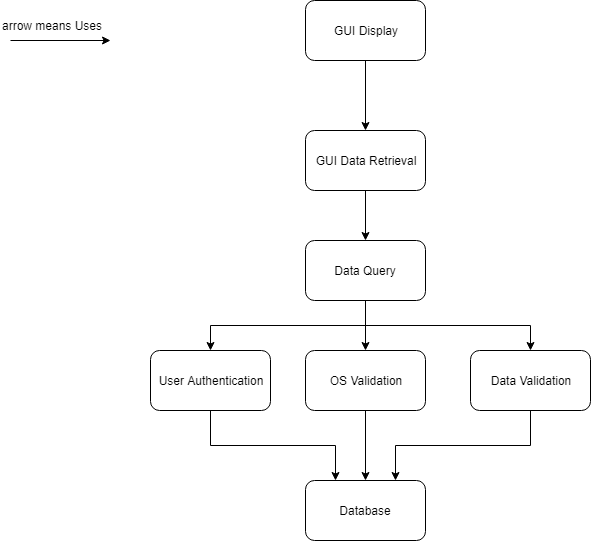
\includegraphics[width=0.7\textwidth]{group33_module_heirarchy.png}
\caption{Use hierarchy among modules}
\label{FigUH}
\end{figure}

%\section*{References}
The Gantt Chart located on the \href{https://gitlab.cas.mcmaster.ca/coitn/se3xa3-fall2017/blob/5f395a201142607bc7222f5af2450baca2cb0a42/Doc/DevelopmentPlan/group33-project-schedule.pdf}{project page} contains individual test role assignments while the Gantt chart below breaks the testing into a set of tasks.
\begin{figure}[H]
\centering
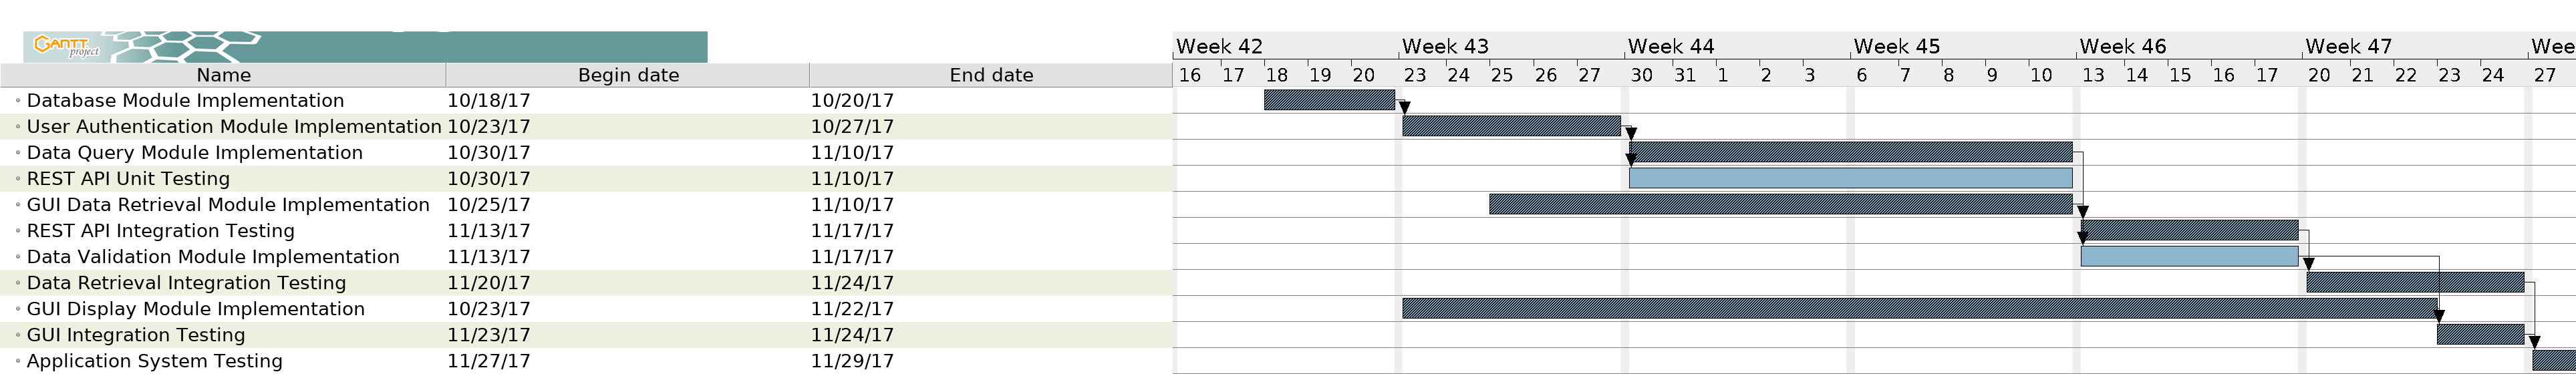
\includegraphics[width=1.0\textwidth]{Group33_SIMS_project_breakdown.png}
\caption{Updated Gantt Chart With Testing}
\label{FigUI}
\end{figure}

\bibliographystyle {plainnat}
\bibliography {MG}

\end{document}
